\documentclass{../llncs}
%%%%%%%%%%%%%%%%%%%%%%%%%%%%%%%%%%%%%%%%%%%%%%%%%%%%%%%%%%%
%% package sillabazione italiana e uso lettere accentate
% \usepackage[latin1]{inputenc}
\usepackage[utf8]{inputenc}
\usepackage[english]{babel}
\usepackage[T1]{fontenc}
%%%%%%%%%%%%%%%%%%%%%%%%%%%%%%%%%%%%%%%%%%%%%%%%%%%%%%%%%%%%%

% per gli elenchi
\usepackage{enumitem}

% https://en.wikibooks.org/wiki/LaTeX/Source_Code_Listings
%%%%%%%%%%%%%%%%%%%%%%%%%%%%
\usepackage{listings}

\usepackage{xcolor}
\definecolor{darkgreen}{HTML}{007700}

\lstset{
	basicstyle=\small\ttfamily,
	columns=fullflexible,
	keywordstyle=\color{violet}\bfseries,
	commentstyle=\color{darkgreen},
	breaklines=true,	 			% sets automatic line breaking
	captionpos=b,					% sets the caption-position to bottom
	stringstyle=\color{blue},     	% string literal style
	showstringspaces=false, 		% no special string spaces
	caption={\lstname},
	% title=\lstname,               % show the filename of files included with \lstinputlisting;
	numbers=left,
	numberstyle=\tiny,
	stepnumber=1,
	numbersep=5pt,
	frame=shadowbox
	% , float=*
}

\lstdefinestyle{style_qa}{
	language=C++,
	morekeywords={
		Plan,System,Event,Dispatch,Context,ip,host,port,httpserver,QActor,context,
		normal,switchTo,transition,whenMsg,finally,repeatPlan,stopAfter,resumeLastPlan,
		onMsg,addRule,replyToCaller,onEvent,removeRule,javaRun,whenTime,sendto,emit,else,not,
		selfMsg,forward,delay,whenEvent,printCurrentEvent,EventHandler,forwardEvent,Rules
	}
}

\lstnewenvironment{qacode}[1][]{\lstset{style=style_qa, #1}}{}
% \begin{qacode}[caption={Programma Blink, "Hello World!"}]
% ...
% \end{qacode}
%%%%%%%%%%%%%%%%%%%%%%%%%%%%

\usepackage{url}
\usepackage{xspace}
\usepackage{color}
\makeatletter
%%%%%%%%%%%%%%%%%%%%%%%%%%%%%% User specified LaTeX commands.
\usepackage{../manifest}

\makeatother

% https://en.wikibooks.org/wiki/LaTeX/Hyperlinks
% LaTeXimpaziente: "Il pacchetto hyperref, che di regola va caricato per ultimo, crea i collegamenti ipertestualivall’interno del documento, rendendo cliccabili i riferimenti incrociati"
\usepackage{hyperref}

%%%%%%%
 \newif\ifpdf
 \ifx\pdfoutput\undefined
 \pdffalse % we are not running PDFLaTeX
 \else
 \pdfoutput=1 % we are running PDFLaTeX
 \pdftrue
 \fi
%%%%%%%
 \ifpdf
 \usepackage[pdftex]{graphicx}
 \else
 \usepackage{graphicx}
 \fi
%%%%%%%%%%%%%%%
 \ifpdf
 \DeclareGraphicsExtensions{.pdf, .jpg, .tif}
 \else
 \DeclareGraphicsExtensions{.eps, .jpg}
 \fi
%%%%%%%%%%%%%%%

\newcommand{\java}{\textsf{Java}}
\newcommand{\android}{\texttt{Android}}
\newcommand{\dsl}{\texttt{DSL}}
\newcommand{\jazz}{\texttt{Jazz}}
\newcommand{\rtc}{\texttt{RTC}}
\newcommand{\ide}{\texttt{Contact-ide}}
\newcommand{\xtext}{\texttt{XText}}
\newcommand{\xpand}{\texttt{Xpand}}
\newcommand{\xtend}{\texttt{Xtend}}
\newcommand{\pojo}{\texttt{POJO}}
\newcommand{\junit}{\texttt{JUnit}}

\newcommand{\action}[1]{\texttt{#1}\xspace}
% \newcommand{\codescript}[1]{{\scriptsize{\texttt{#1}}}\xspace}
\newcommand{\codescript}[1]{{\mbox{\small{\texttt{#1}}}}\xspace}
\newcommand{\code}[1]{{\color{blue}\small{\texttt{#1}}}}
\newcommand{\fname}[1]{{\small{\color{magenta}\texttt{#1}}}}
\newcommand{\node}{\textsf{NodeJs}}
\newcommand{\qa}{\textsf{\textit{QActor}}\xspace}

% Cross-referencing
\newcommand{\labelsec}[1]{\label{sec:#1}}
\newcommand{\xs}[1]{\sectionname~\ref{sec:#1}}
\newcommand{\xsp}[1]{\sectionname~\ref{sec:#1} \onpagename~\pageref{sec:#1}}
\newcommand{\labelssec}[1]{\label{ssec:#1}}
\newcommand{\xss}[1]{\subsectionname~\ref{ssec:#1}}
\newcommand{\xssp}[1]{\subsectionname~\ref{ssec:#1} \onpagename~\pageref{ssec:#1}}
\newcommand{\labelsssec}[1]{\label{sssec:#1}}
\newcommand{\xsss}[1]{\subsectionname~\ref{sssec:#1}}
\newcommand{\xsssp}[1]{\subsectionname~\ref{sssec:#1} \onpagename~\pageref{sssec:#1}}
\newcommand{\labelfig}[1]{\label{fig:#1}}
\newcommand{\xf}[1]{\figurename~\ref{fig:#1}}
\newcommand{\xfp}[1]{\figurename~\ref{fig:#1} \onpagename~\pageref{fig:#1}}
\newcommand{\labeltab}[1]{\label{tab:#1}}
\newcommand{\xt}[1]{\tablename~\ref{tab:#1}}
\newcommand{\xtp}[1]{\tablename~\ref{tab:#1} \onpagename~\pageref{tab:#1}}
% Category Names
\newcommand{\sectionname}{Section}
\newcommand{\subsectionname}{Subsection}
\newcommand{\sectionsname}{Sections}
\newcommand{\subsectionsname}{Subsections}
\newcommand{\secname}{\sectionname}
\newcommand{\ssecname}{\subsectionname}
\newcommand{\secsname}{\sectionsname}
\newcommand{\ssecsname}{\subsectionsname}
\newcommand{\onpagename}{on page}

\newcommand{\xauthA}{Filippo Frabetti}
\newcommand{\xauthB}{Nicola Semprini}
\newcommand{\xauthC}{Paolo Magnani}
\newcommand{\xfaculty}{II Faculty of Engineering}
\newcommand{\xunibo}{Alma Mater Studiorum -- University of Bologna}
\newcommand{\xaddrBO}{viale Risorgimento 2}
\newcommand{\xaddrCE}{via Venezia 52}
\newcommand{\xcityBO}{40136 Bologna, Italy}
\newcommand{\xcityCE}{47023 Cesena, Italy}

%
% Comments
%
% What’s wrong with \bf, \it, etc.? --> https://texfaq.org/FAQ-2letterfontcmd
% \newcommand{\todo}[1]{\bf{TODO:}\emph{#1}}
\newcommand{\todo}[1]{\textbf{TODO:} \emph{#1}}

\begin{document}

\title{Software Systems Engineering: Final task 2018}

\author{\xauthA, \xauthB, \xauthC}

\institute{%
  \xunibo\\\xaddrBO, \xcityBO\\
  \email{filippo.frabetti@studio.unibo.it}\\
  \email{nicola.semprini4@studio.unibo.it}\\
  \email{paolo.magnani5@studio.unibo.it}
}

\maketitle

% %%%%%%%%%%%%%%%%%%%%%%%% ABSTRACT + KEYWORDS - TODO... %%%%%%%%%%%%%%%%%%%%%%%%
\begin{abstract}
\footnotesize

This document is the explicit representation of the production process adopted.\\

\todo{abstract and keywords}

% (This part is optional)
%%This a Latex template to be used for the explicit representation of the production process adopted in the Software Systems Engineering course. 
% THIS DOCUMENT MUST FILL AT MOST TWO PAGES AND MUST BE PRINTED ON A SINGLE PAPER SHEET.

% The document can be compiled by using the \fname{kitISLatex.zip} given in \code{iss2018/it.unibo.issMaterial/issdocs/Lab}
  
\keywords{
% (This part is optional)
Software engineering, software development process, process representation, ...
}
\end{abstract}

% evita le righe eccessivamente lunghe aumentando la spaziatura tra le parole
% Il comando \fussy ripristina le impostazioni predefinite 
\sloppy

%===========================================================================
\section{Introduction}
\labelsec{intro}
%===========================================================================

%===========================================================================
\section{Vision}
\labelsec{vision}

Scegliamo di procedere top-down, con zooming progressivo verso i dettagli.
%=========================================================================== 

%===========================================================================
\section{Requirements}
\labelsec{Requirements}

%With reference to a \texttt{mbot} physical robot working in a virtual environment, build an application that sends the data sensed by the virtual and the real sonars to the radar. More specifically:
%\begin{itemize}
%\item[-]the data of the \emph{virtual sonar} \texttt{sonar1} must be displayed on the direction of angle=\fname{30};
%\item[-]the data of the \emph{virtual sonar} \texttt{sonar2} must be displayed on the direction of angle=\fname{120};
%\item[-]the data of the \emph{virtual sonar} on the virtual robot must be displayed on the direction of angle=\fname{90} at the fixed distance of \fname{40};
%\item[-]the data of the \emph{real sonar} on the physical robot must be displayed on the direction of angle=\fname{0};
%\end{itemize}

% 13 - A new problem
%\begin{enumerate}
%\item The physical robot must expose in a visible way a \code{Led} and:
%\begin{itemize}
%\item[-] the Led must be \code{on} when the robot is engaged by an user (human or machine);
%\item[-] the Led must be \code{off} when the robot is available for booking.
%\end{itemize}
%\item the robot system does not expose any public available usage interface;
%\item in order to use the robot, an user must first of all send 'to the system' a \code{booking request}. The system
%must return an answer including an \code{access token} if the robot is available. If the answer is negative, (robot
%already engaged) and the request includes a '\texttt{notify-me flag}', the system must notify the user when to robot
%becomes again available;
%\item the user that receives the \code{access token} must send within a given \code{acquisition-deadline} (e.g. \code{30 sec}) the request for a \emph{robot-driving command interface}, by appending to the request the \code{access token}. If the
%\emph{acquisition-deadline} expires, the robot returns in its 'available state';
%\item the user can use the \emph{robot-driving command interface} at most for a prefixed \code{usage-duration} time;
%\item the user can explicitly release the robot resource by sending a \code{booking release} message;
%\item if many users attempt to book the robot resource 'at the same time', the system could operate in two different
%ways:
%\begin{itemize}
%\item[(a)] by selecting the first \emph{emitted} request;
%\item[(b)] by selecting the first \emph{received} request
%\end{itemize}
%\end{enumerate}

% FINAL TASK 2018
In a home of a given city (e.g. Bologna), a \texttt{ddr} robot is used to clean the floor of a room (\code{R-FloorClean}).

The floor in the room is a flat floor of solid material and is equipped with two \emph{sonars}, named \code{sonar1} and \code{sonar2} as shown in the picture (\code{sonar1} is that at the top). The initial position (\code{start-point}) of the robot is detected by \code{sonar1}, while the final position (\code{end-point}) is detected by \code{sonar2}.\\

\noindent The robot works under the following conditions:
\begin{enumerate}
\item \code{R-Start}: an \code{authorized user} has sent a \texttt{START} command by using a human \texttt{GUI} interface (\code{console}) running on a conventional PC or on a smart device (\texttt{Android}).
\item \code{R-TempOk}: the value temperature of the city is not higher than a prefixed value (e.g. \texttt{25} degrees Celsius).
\item \code{R-TimeOk}: the current clock time is within a given interval (e.g. between \texttt{7} a.m and \texttt{10} a.m).
\end{enumerate}

\noindent While the robot is working:
\begin{itemize}[label={--}]
\item it must blink a \texttt{Led} put on it, if the robot is a \fname{real} robot (\code{R-BlinkLed}).
\item it must blink a \texttt{Led Hue Lamp} available in the house, if the robot is a \fname{virtual} robot (\code{R-BlinkHue}).
\item it must avoid fixed obstacles (e.g. furniture) present in the room (\code{R-AvoidFix}) and/or mobile obstacles like
balls, cats, etc. (\code{R-AvoidMobile}).
\end{itemize}

Moreover, the robot must stop its activity when one of the following conditions apply:
\begin{enumerate}
\item \code{R-Stop}: an \code{authorized user} has sent a \texttt{STOP} command by using the \code{console}.
\item \code{R-TempKo}: the value temperature of the city becomes higher than the prefixed value.
\item \code{R-TimeKo}: the current clock time is beyond the given interval.
\item \code{R-Obstacle}: the robot has found an obstacle that it is unable to avoid.
\item \code{R-End}: the robot has finished its work.
\end{enumerate}

%During its work, the robot can optionally:
%\begin{itemize}[label={--}]
%\item \code{R-Map}: build a map of the room floor with the position of the fixed obstacles. Once built, this map can be
%used to define a plan for an (optimal) path form the \code{start-point} to the \code{end-point}.
%\end{itemize}
%
%Other requirements:
%\begin{enumerate}
%\item The work can be done by a team composed of \code{NT} people, with \code{1<=NT<=4}.
%\item If \code{NT>1}, the team must explicitly indicate the work done by each component.
%\item If \code{NT==4}, the requirement \code{R-Map} is mandatory.
%\end{enumerate}
%===========================================================================

%===========================================================================
\section{Requirement analysis}
\labelsec{ReqAnalysis}
Dai requisiti emerge il fatto che il sistema sia distribuito e composto da due nodi di esecuzione: uno per il robot e uno che ospita la logica di controllo e la console per pilotare il robot (\code{R-Start} e \code{R-Stop}).\\

\noindent Si delineano nello specifico 5 entità:
\begin{enumerate}
\item il robot, che può essere sia fisico sia virtuale (\texttt{RealDDR} e \texttt{VirtualDDR}), e l'ambiente in cui si muove (fisico/virtuale)
\item gli attuatori: il \texttt{Led} per il robot reale e l'\texttt{Hue Lamp} remota per quello virtuale
\item i sensori: un indicatore di temperatura remoto (\texttt{TemperatureSensor}) e un orologio (\texttt{Clock})
\item un utilizzatore umano (\texttt{HumanOperator}) della \code{console}
\item più un componente che andrà ad incapsulare l'\texttt{Application logic}
\end{enumerate}

\noindent L'ambiente è inoltre costituito a sua volta da:
\begin{itemize}[label={--}]
\item 2 sensori \code{sonar1} e \code{sonar2} (ambiente virtuale)
\item ostacoli fissi (pareti) e mobili
\end{itemize}

L'architettura del sistema può essere descritta in maniera informale dalla \xf{informalRA}.
\begin{figure}[!htb]
\centering
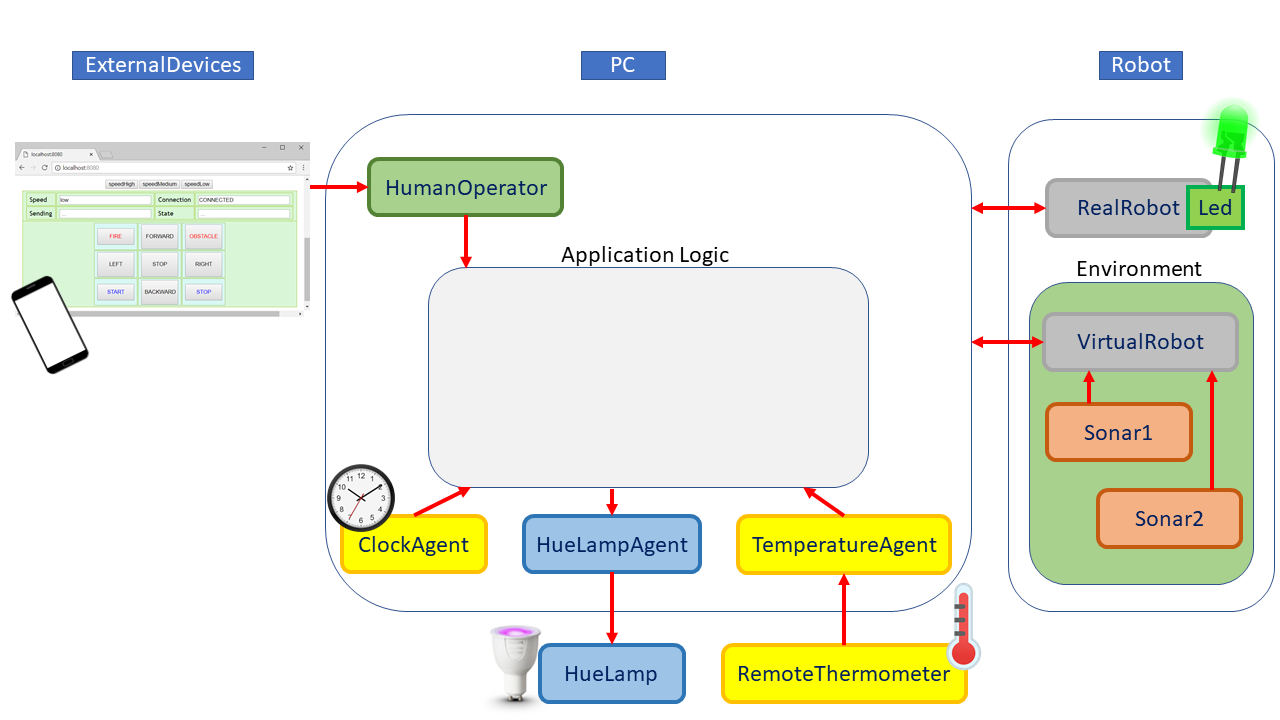
\includegraphics[scale=0.4]{img/informalArchitecture1.png}
\caption{Architettura informale ottenuta dall'analisi dei requisiti}\labelfig{informalRA}
\end{figure}

\subsection{Actuators}
\labelssec{actuatorsRA}
Il \texttt{Led}, essendo un componente estremamente semplice e trovandosi sul robot fisico, può essere visto come un'entità passiva senza un proprio flusso di controllo. Pertanto, il modello del \texttt{Led} -- un oggetto Java -- può essere formalmente definito dalla seguente interfaccia:

\begin{center}
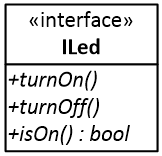
\includegraphics[scale=0.4]{img/iled.png}
\end{center}

L'interazione con il \texttt{Led} può quindi avvenire tramite \textit{procedure call} ad opera del robot fisico su cui si trova.\\

L'\texttt{Hue Lamp} è invece un'entità attiva che ci viene fornita dal committente insieme ad un componente software per poter interagire con essa attraverso un'interfaccia \textit{RESTful}
\footnote{\url{https://www.developers.meethue.com/philips-hue-api}}.

Possiamo quindi definire il modello di un attore in grado di interagire con l'\texttt{Hue Lamp} remota: per farlo usiamo il linguaggio custom della nostra Software House \qa, poiché ci permette di modellare sistemi distribuiti eterogenei.\\

\lstinputlisting[style=style_qa, firstline=15, lastline=34, firstnumber=15]{../it.unibo.finalTask2018/src/requirementsAnalysis.qa}

Si noti come la scelta di utilizzare l'evento \codescript{lightCmd} consenta di controllare più dispositivi senza che questi siano noti a priori dalla sorgente che emette tali eventi in base alla logica applicativa.

Inoltre, poiché i comandi utilizzati nel payload dell'evento non si limitano solo a gestire il \textit{lampeggiamento}, il modello è generale e facilmente riutilizzabile. Ad esempio un cambiamento dei requisiti potrebbe stabilire che il led vada solo acceso durante il movimento del robot.

\subsection{Sensors}

\subsubsection{TemperatureSensor}
Poiché abbiamo a che fare con un servizio remoto che fornisce i dati sulla temperatura, ci viene naturale modellare un attore che funga da adapter per permettere la comunicazione di questi con il sistema.

Nello specifico, l'applicazione può interagire con l'adapter mediante tre possibili approcci:
\begin{itemize}
\item \textbf{polling:} chi necessita dell'informazione a farsi carico di fare richiesta periodicamente al sensore;
\item \textbf{pattern observer:} l'observer si registra presso l'observable e viene notificato al cambiamento di stato di quest'ultimo;
\item \textbf{publish/subscribe:} è il sensore stesso a pubblicare all'esterno le informazioni quando queste sono disponibili ad uso degli eventuali subscriber.
\end{itemize}
Scegliamo di adottare la terza strategia, poiché meno costosa in termini di dati scambiati e poiché garantisce un minor accoppiamento tra le entità coinvolte.

Anche in questo caso l'adapter del sensore, non conoscendo i componenti interessati, emette un evento \codescript{temperature : temperature(T)} che può essere percepito da chiunque sia in ascolto.\\

\lstinputlisting[style=style_qa, firstline=38, lastline=52, firstnumber=38]{../it.unibo.finalTask2018/src/requirementsAnalysis.qa}

\subsubsection{Clock}
Poiché nei requisiti non viene specificata la natura del \texttt{Clock}, scegliamo di modellarlo come un attore a se stante -- separato dalla logica applicativa specifica del problema -- così che in futuro possa essere facilmente introdotto un qualsiasi meccanismo di sincronizzazione distribuito (es. orologio logico di Lamport
\footnote{\url{https://en.wikipedia.org/wiki/Leslie_Lamport}}).

\lstinputlisting[style=style_qa, firstline=56, lastline=71, firstnumber=56]{../it.unibo.finalTask2018/src/requirementsAnalysis.qa}

Il suo comportamento interno è pressoché analogo a quello visto per il \texttt{TemperatureSensor}.

\subsection{HumanOperator}
Lo \texttt{HumanOperator} può essere modellato come un emettitore di comandi per il robot. Per disaccoppiare le comunicazioni tra sorgente e destinatario dei comandi, l'operator si rivolge ad una terza entità che rappresenta la logica applicativa, così da non essere vincolato a conoscere l'identità di ogni possibile robot pilotabile.\\

\lstinputlisting[style=style_qa, firstline=75, lastline=89, firstnumber=75]{../it.unibo.finalTask2018/src/requirementsAnalysis.qa}

Lo \texttt{HumanOperator} dovrà inoltre fornire un'interfaccia grafica per permettere l'interazione con l'utente da qualsiasi dispositivo (\code{R-Start}). Ciò può essere realizzato in prima battuta tramite l'inserimento del flag \codescript{-httpserver} nel contesto dell'applicazione, sfruttando il server HTTP fornito dall'infrastruttura \qa, con l'idea di poterlo sostituire in futuro con un server più sofisticato.\\

\lstinputlisting[style=style_qa, firstline=12, lastline=12, firstnumber=12]{../it.unibo.finalTask2018/src/requirementsAnalysis.qa}

\subsection{Robot}
Ci viene fornito un modello del robot espresso nel linguaggio \qa
\footnote{it.unibo.mbot.divide/src/realRobotExecutor.qa}: questi è in grado di ricevere messaggi \codescript{moveRobot : moveRobot(CMD)} e di interpretarli come comandi di movimento (stop, forward, left, right, backward).

Il robot è anche dotato di un sonar frontale che gli permette di rilevare la presenza di ostacoli (\code{R-AvoidFix} e \code{R-AvoidMobile}). Il robot riveste quindi il duplice ruolo di attuatore e di sensore, in quanto emette informazioni relative alla distanza dagli ostacoli che incontra sotto forma di eventi \codescript{frontSonar : sonar(DISTANCE)}.\\

Il robot è quindi un'entità attiva il cui scopo è interpretare i messaggi ricevuti in un certo formato ed emettere eventi relativi al sonar frontale. L'implementazione delle varie mosse è delegata ad un'opportuna classe Java che può essere modificata senza alterare il modello del robot.\\

\lstinputlisting[style=style_qa]{../it.unibo.finalTask2018/src/ddr.qa}

\vspace{8px}

Nell'ambiente virtuale sono presenti due sonar in grado di rilevare la presenza di un robot che passi in corrispondenza di uno dei due. Per questo motivo definiamo un ulteriore evento \codescript{sonarSensor : sonar(NAME, DISTANCE)}, dove \codescript{NAME} è \code{sonar1} o \code{sonar2}.\\

Da notare come l'emissione di tali eventi dipenda dalla specifica implementazione del \textit{virtual environment} (le operazioni ad esso relative sono delegate ad una classe Java):

\lstinputlisting[language=Java, firstline=8, lastline=19, firstnumber=8]{../it.unibo.finalTask2018/src/it/unibo/finalTask2018/robot/MockRobot.java}

\subsection{Application logic}
L'immagine della \xf{informalRA} può essere quindi formalmente definita dal seguente sistema {\qa}:\\

\lstinputlisting[style=style_qa, lastline=13]{../it.unibo.finalTask2018/src/requirementsAnalysis.qa}

\vspace{8px}

\lstinputlisting[style=style_qa, firstline=93, lastline=116, firstnumber=93]{../it.unibo.finalTask2018/src/requirementsAnalysis.qa}

\vspace{8px}

Poiché abbiamo utilizzato un \emph{modello eseguibile}, questo ci fornisce anche un primo \textbf{prototipo} funzionante della nostra applicazione.
%===========================================================================

%===========================================================================
\section{Problem analysis}
\labelsec{ProblemAnalysis}
Il problema definito dai requisiti si colloca nell'ambito dell'IoT, dove è diffuso l'utilizzo della cosiddetta \emph{architettura esagonale} come design pattern per gestire il rapporto tra input, elaborazione ed output nei sistemi distribuiti. Un ruolo centrale viene rivestito dalla business logic e dal modello delle risorse (\emph{Resource Model}), mentre gli altri componenti del sistema vengono visti tramite degli adapter verso le varie tecnologie ed implementazioni.\\

Il modello delle risorse è un disaccoppiatore del mondo fisico dal mondo della logica applicativa, che deve essere indipendente dalla tecnologia. Nello specifico:
\begin{enumerate}
\item un cambiamento del sensore fisico causa un cambiamento nello stato del modello del sensore stesso
\item al cambiamento del modello, l'informazione viene notificata al controller (è un observer del modello)
\item il controller modifica quindi il modello dell'attuatore in base alla logica applicativa
\item l'aggiornamento del modello dell'attuatore comporta infine un aggiornamento dell'attuatore fisico
\end{enumerate}

Come analisti riteniamo vantaggioso introdurre un modello delle risorse così da non vincolare la logica applicativa a dettagli tecnologico-implementativi, sebbene ciò comporti un piccolo sforzo aggiuntivo iniziale. Tale overhead è però un investimento a fronte dello sviluppo futuro di applicazioni simili, inoltre, se il modello fosse standardizzato, sarebbe garantita l'interoperabilità tra sistemi diversi.

\subsection{Resource Model}
Per la definizione del modello delle risorse usiamo un linguaggio dichiarativo che consenta di esprimere sia lo stato di ciascun componente, sia le operazioni primitive su di esso. A tal fine, introduciamo il seguente modello scritto in Prolog:\\

\lstinputlisting[language=Prolog, keywordstyle=\color{black}]{../it.unibo.finalTask2018/resourceModel.pl}

\subsection{Logical architecture}
In seguito all'introduzione del \emph{Resource Model} possiamo definire l'architettura logica del sistema in modo informale tramite la \xf{informalLA}.

\begin{figure}[!htb]
\centering
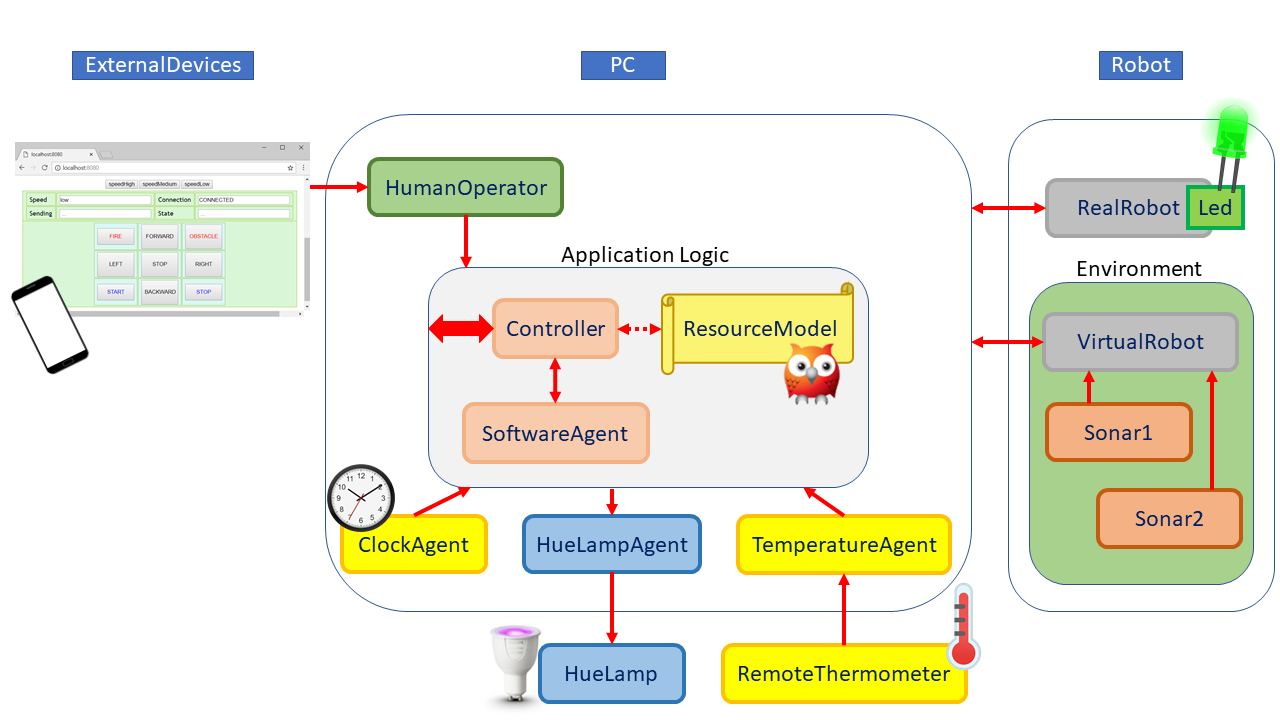
\includegraphics[scale=0.4]{img/informalArchitecture2.png}
\caption{Architettura logica informale}\labelfig{informalLA}
\end{figure}

Rispetto all'architettura risultante dall'analisi dei requisiti, sono stati inoltre aggiunti i componenti \texttt{Controller} e \texttt{SoftwareAgent}.

\subsection{Controller}
Il ruolo del \texttt{Controller} è quello di gestire il modello delle risorse in base agli eventi ricevuti dai sensori e alla logica applicativa. Ci viene naturale utilizzare il pattern MVC: Resource Model, sensori/attuatori e Controller.

Modelliamo il \texttt{Controller} come un attore in grado di ricevere informazioni di input dagli altri componenti del sistema (vedi righe 3-9) ed emettere comandi di output sotto forma di eventi \codescript{ctrlEvent : ctrlEvent(CATEG,NAME,CMD)}.\\

\lstinputlisting[style=style_qa, lastline=18]{../it.unibo.finalTask2018/src/problemAnalysis.qa}

Tramite un \emph{EventHandler} ogni evento emesso dai sensori viene mappato in un evento \codescript{inputCtrlEvent : inputEvent( CATEG, NAME, VALUE )} ad uso interno del \texttt{Controller}. In questo modo gli eventi provenienti da sensori fisici diversi vengono trattati allo stesso modo e non vengono mai persi (a meno che le operazioni compiute dal \texttt{Controller} non richiedano troppo tempo), essendo l'\emph{EventHandler} un componente event-driven. Per discriminare la natura di questi eventi vengono usati i campi \codescript{CATEG} e \codescript{NAME} presenti nel payload.

Ad ogni modifica del Resource Model relativa allo stato di un attuatore, il \texttt{Controller} emette a sua volta degli eventi \codescript{ctrlEvent} per notificare il cambiamento ai vari attuatori fisici.\\

\lstinputlisting[style=style_qa, firstline=26, lastline=118, firstnumber=26]{../it.unibo.finalTask2018/src/problemAnalysis.qa}

Attualmente sono soddisfatti i requisiti \code{R-TempOk} e \code{R-TimeOk} in quanto il \texttt{Controller} blocca ogni modifica allo stato del robot al di fuori di un certo intervallo temporale o in presenza di temperature troppo elevate. Il robot viene inoltre fermato non appena queste condizioni non sono più verificate (\code{R-TempKo} e \code{R-TimeKo}).

Oltre a questo, sono anche soddisfatti i requisiti relativi al lampeggiamento del \texttt{Led} e della \texttt{HueLamp} (\code{R-BlinkLed} e \code{R-BlinkHue}), dal momento che alla modifica del modello del robot segue l'emissione di un opportuno evento \codescript{ctrlEvent} ad uso degli attuatori della categoria \emph{''led''}.

\subsection{Software Agent}
Il \texttt{SoftwareAgent} realizza la logica applicativa in collaborazione col \texttt{Controller}, occupandosi di manovrare il robot secondo il vincolo \code{R-FloorClean}. Decidiamo quindi di modellarlo come un attore nel suo stesso contesto.

L'agent si mette in ascolto degli eventi provenienti dai vari sonar e invia opportuni messaggi \codescript{cmd} al controller, gli stessi utilizzati dallo \texttt{HumanOperator} per muovere il robot.\\

In una fase preliminare, per motivi di testing, il \texttt{SoftwareAgent} fa semplicemente ruotare il robot quando esso viene rilevato dai sonar a distanza ravvicinata.\\

\lstinputlisting[style=style_qa, firstline=122, lastline=171, firstnumber=122]{../it.unibo.finalTask2018/src/problemAnalysis.qa}

\subsection{Changes to HumanOperator}
Rispetto al modello precedente, la \emph{web GUI} realizzata tramite il flag \codescript{-httpserver} è stata dotata di bottoni che, quando vengono premuti, scatenano eventi \codescript{usercmd : usercmd(X)}. Lo \texttt{HumanOperator} cattura questi eventi e li inoltra sotto forma di messaggi \codescript{cmd : cmd(X)} al \texttt{Controller}.

Lo \texttt{HumanOperator} è ancora un emettitore di comandi per il robot come visto nella sezione precedente, tuttavia ora è in grado di generarli in base ai pulsanti premuti dall'utilizzatore umano sulla console.\\

\lstinputlisting[style=style_qa, firstline=175, lastline=191, firstnumber=175]{../it.unibo.finalTask2018/src/problemAnalysis.qa}

L'attuale \emph{GUI} in futuro potrà essere sostituita da un'implementazione differente per soddisfare i requisiti \code{R-Start} e \code{R-Stop}.

\subsection{Virtual Robot with Node.js}
Il robot virtuale si mette in attesa di messaggi \codescript{moveRobot} e li interpreta come comandi di movimento, tuttavia i cambiamenti nel modello del robot vengono notificati all'esterno sotto forma di eventi \codescript{ctrlEvent}.

Per effettuare la conversione da \codescript{ctrlEvent} a messaggi abbiamo utilizzato un \emph{EventHandler}: questo permette di accodare gli eventi senza il rischio di perderne qualcuno (il robot virtuale è quindi, nel suo complesso, un componente \emph{event-driven}).\\

\lstinputlisting[style=style_qa, lastline=13]{../it.unibo.finalTask2018/src/virtualRobotNode.qa}

Poichè gli \emph{EventHandler} possono solo convertire eventi in messaggi con lo stesso payload, introduciamo l'attore \texttt{nodebroker}, il cui compito è quello di convertire i messaggi \codescript{ctrlMsg : ctrlEvent(CATEG, NAME, CMD)} inviati dall'\emph{EventHandler} in messaggi \codescript{moveRobot : moveRobot(CMD)} per il robot virtuale.\\

\lstinputlisting[style=style_qa, firstline=52, lastline=57, firstnumber=52]{../it.unibo.finalTask2018/src/virtualRobotNode.qa}

\subsection{Real Robot with a mock object}
Per quanto riguarda il robot fisico, al momento viene simulato tramite un attore che usa un oggetto Java, il quale si limita a stampare a video i comandi ricevuti. Tale attore deve anche gestire il lampeggiamento del led che sarà collocato sul robot fisico: nel rispetto delle considerazioni fatte durante l'analisi dei requisiti, questi viene visto attraverso l'interfaccia Java precedentemente definita (\xss{actuatorsRA}).

Il modello di questo robot è quindi equivalente a quello del robot virtuale, discostandosi unicamente per l'implementazione dei metodi della classe Java utilizzati per realizzare le varie mosse.\\

\lstinputlisting[language=Java, firstline=11, lastline=36, firstnumber=11]{../it.unibo.finalTask2018/src/it/unibo/finalTask2018/robot/RealRobotMock.java}

Da notare come entrambi i robot, reagendo agli stessi eventi \codescript{ctrlEvent} generati al cambiamento del modello del robot, possono eseguire in contemporanea le medesime mosse.

\subsection{Changes to HueLampAgent}
Come per il robot, anche il modello della \texttt{HueLamp} dev'essere aggiornato per poter lavorare con gli eventi \codescript{ctrlEvent} emessi dal controller. Analogamente a quanto fatto prima, abbiamo utilizzato un \emph{EventHandler} per convertire tali eventi in \codescript{lightCmd}, ovvero nel formato degli eventi gestiti dalla lampada.\\

\lstinputlisting[style=style_qa, firstline=19, lastline=23, firstnumber=19]{../it.unibo.finalTask2018/src/problemAnalysis.qa}

Il resto del modello non ha subito variazioni rispetto a quello precedentemente mostrato. L'attuale implementazione della classe Java che viene utilizzata (tramite \codescript{javaRun}) non è altro che un oggetto mock che mostra un'interfaccia grafica in grado di ''lampeggiare''.
%===========================================================================

%===========================================================================
\section{Project}
\labelsec{Project}
Al momento, l'applicazione è in grado di soddisfare i seguenti requisiti:
\begin{itemize}
\item \code{R-TempOk}, \code{R-TimeOk}, \code{R-TempKo} e \code{R-TimeKo}, ad opera di opportune regole Prolog presenti nella base di conoscenza del \texttt{Controller}
\item \code{R-BlinkLed} e \code{R-BlinkHue}
\footnote{Resta da sviluppare l'implementazione della classe Java \emph{technology-dependent} che dovrà interagire in modo RESTful con la \texttt{Hue Lamp} remota}, mediante l'emissione da parte del controller di eventi \codescript{ctrlEvent : ctrlEvent(led,l1,CMD)} a seguito della modifica del modello del led \codescript{l1} in base allo stato di movimento del robot
\end{itemize}

Rimangono da affrontare i restanti requisiti relativi al movimento autonomo del robot (pilotato da \texttt{SoftwareAgent}):
\begin{enumerate}
\item \code{R-Start} e \code{R-Stop}: la pulizia della stanza inizia e termina preventivamente a seguito di un comando \texttt{start/stop} inviato da un \emph{utente autorizzato}
\item \code{R-FloorClean} e \code{R-End}: il robot deve pulire l'intera superficie della stanza (da \code{sonar1} a \code{sonar2}), fermandosi al termine del lavoro
\item \code{R-AvoidMobile}, \code{R-AvoidFix} e \code{R-Obstacle}: il robot deve essere in grado di rilevare ed evitare gli ostacoli sia fissi sia mobili, eventualmente fermandosi nel caso ciò non sia possibile
\end{enumerate}

\subsection{Starting and stopping the agent}
Al momento è disponibile una \emph{web GUI} fornita dall'infrastruttura \qa grazie alla presenza del flag \codescript{-htthserver} presente nel contesto dell'applicazione. Questa è in grado di emettere eventi \codescript{usercmd : usercmd(CMD)} alla pressione dei pulsanti di movimento da parte dell'utilizzatore umano.

Oltre ai bottoni che corrispondono ai movimenti elementari del robot, ve ne sono altri due che possono essere utilizzati per gestire l'avvio e la terminazione della pulizia della stanza ad opera di \texttt{SoftwareAgent}, con l'idea di gestire in seguito la problematica relativa all'autenticazione degli utenti.

Attualmente, la GUI di default emettere eventi \codescript{cmd : cmd(C)} alla pressione di questi pulsanti. Abbiamo però deciso di sostituirli con eventi \codescript{alarm : usercmd(C)} così che, avendo lo stesso payload degli altri, la loro gestione risulti semplificata.\\

Poiché non vogliamo che nessun comando vada perso, introduciamo un componente event-driven (\emph{EventHandler}) che effettui un mapping degli eventi \codescript{usercmd} ed \codescript{alarm} in messaggi \codescript{externalcmd} diretti all'agent e aventi lo stesso payload dei precedenti.

\subsubsection{R-Start e R-Stop}
Alla pressione del pulsante di start, il robot deve trovarsi vicino a \code{sonar1} per poter partire con la pulizia, in caso contrario il comando viene ignorato. Se invece viene ricevuto un messaggio di stop (\codescript{usercmd(halt)}) durante il movimento del robot, questi deve fermarsi e l'agent deve ritornare nello stato iniziale.\\

\begin{qacode}[caption={SoftwareAgent, pt1}]
Plan init normal [         
   	println("swAgent start: waiting for start command")
]
transition stopAfter 3600000
	whenMsg externalcmd -> receivedCmd
finally repeatPlan

Plan receivedCmd [
	// R-Start
	onMsg externalcmd : usercmd(start) -> {
   		println("ricevuto usercmd(start)");
   		addRule startCmd
	};
	// R-Stop
   	onMsg externalcmd : usercmd(halt) -> println("ricevuto usercmd(halt)")
]
transition whenTime 800 -> init
	whenEvent [ ?? startCmd ] sonarSensor -> detectedBySonar
\end{qacode}

Se la posizione corrente è in prossimità di \code{sonar1}, ci aspettiamo di ricevere da questi un evento \codescript{sonarSensor} con una distanza inferiore ad una certa soglia. Nel caso invece nessun evento venga rilevato entro un timeout, assumiamo di non essere allineati con un sonar, e quindi sicuramente di non trovarci nella posizione iniziale.\\

\begin{qacode}[caption={SoftwareAgent, pt2}]
Plan detectedBySonar [
	println("detected by a sonar");
	onEvent sonarSensor : sonar(sonar1,D) -> addRule sonarDetect(sonar1,D);
	
	[ !? isCloseTo(sonar1) ] {
		println("close to sonar1");
		selfMsg swagmsg : cmd(clean) // R-Start
	}
	else
		println("NOT close to sonar1!");
		
	removeRule sonarDetect(sonar1,D)
]
transition whenTime 800 -> init
	whenMsg swagmsg -> cleaning
\end{qacode}

La vicinanza ad un sonar viene valutata grazie alle seguenti regole Prolog presenti nella base di conoscenza dell'agent:\\

\begin{lstlisting}[language=Prolog, keywordstyle=\color{black}, caption={SoftwareAgent, Rules - pt1}]
isCloseTo(S) :-
		sonarDetect(S,D),
		eval(gt,D,0),!,
		eval(lt,D,5).
	
isCloseTo(S) :-
		sonarDetect(S,D),
		eval(minus,0,D,R),
		eval(lt,R,5).
\end{lstlisting}

Se durante la pulizia arriva il comando \codescript{externalcmd : usercmd(halt)}, l'agent transita prima in \codescript{receivedCmd} e successivamente nello stato iniziale, in attesa di nuovi comandi.

Ciò avviene anche quando l'utente preme un qualsiasi altro bottone della GUI, riprendendo il controllo manuale del robot.\\

\begin{qacode}[caption={SoftwareAgent, pt3}]
Plan cleaning [
	println("cleaning")
	// do something
]
transition stopAfter 3600000 
	whenEvent frontSonar -> handleFront,
	whenEvent sonarSensor -> detectedByFinal,
	whenMsg externalcmd -> receivedCmd
finally repeatPlan
\end{qacode}

\subsubsection{R-End}
Se durante il suo lavoro il robot viene rilevato in prossimità di \code{sonar2}, possiamo assumere che abbia terminato la pulizia della stanza e che pertanto debba essere fermato. Ciò è possibile reagendo, nello stato di \emph{cleaning}, agli eventi generati dai sonar e transitando in un nuovo stato (\codescript{detectedByFinal}) il cui compito è quello di accertarsi che il robot si trovi effettivamente vicino al secondo sonar, similmente a quanto accade in \codescript{detectedBySonar} per \code{sonar1}.\\

\begin{qacode}[caption={SoftwareAgent, pt4}]
// R-End
Plan detectedByFinal [
	println("detected by a sonar");
	onEvent sonarSensor : sonar(sonar2,D) -> addRule sonarDetect(sonar2,D);

	[ !? isCloseTo(sonar2) ] {
		println("close to sonar2");
		selfMsg swagmsg : cmd(halt) // R-End
	}
	else
		println("NOT close to sonar2!");
		
	removeRule sonarDetect(sonar2,D)
]
transition whenTime 800 -> cleaning
	whenMsg swagmsg -> init
\end{qacode}

\vspace{16px}

Il comportamento di \texttt{SoftwareAgent}, per quanto riguarda il soddisfacimento dei vincoli \code{R-Start}, \code{R-Stop} e \code{R-End}, può essere quindi schematizzato dal diagramma degli stati della \xf{fsmStartStopEnd}.

\begin{figure}[!htb]
\centering
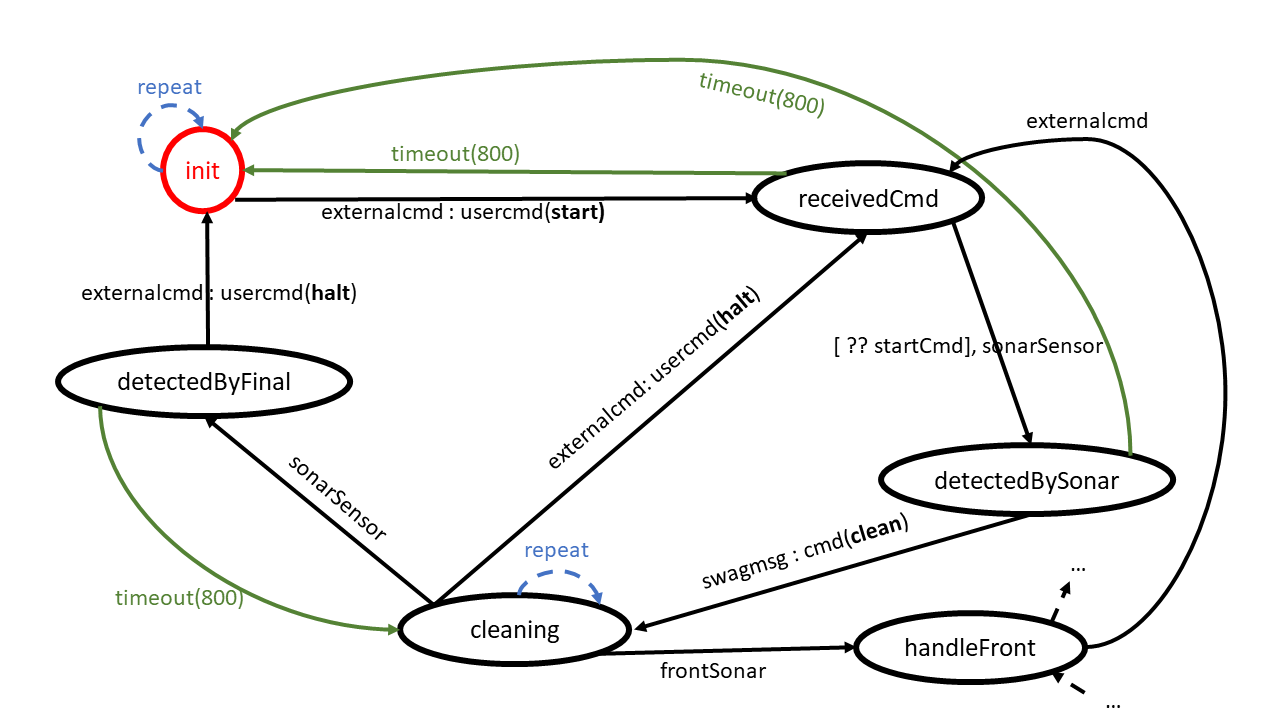
\includegraphics[scale=0.4]{img/swag1.png}
\caption{Diagramma parziale degli stati di \texttt{SoftwareAgent}}\labelfig{fsmStartStopEnd}
\end{figure}

\subsection{Cleaning the room}
Durante la sua attività, il robot deve pulire l'intera superficie della stanza (\code{R-FloorClean}). Concettualmente possiamo identificare 3 macro-stati in cui l'agent può trovarsi: uno stato iniziale in cui attende il comando di start e controlla se le condizioni ad esso relative sono soddisfatte, uno stato di lavoro nel quale effettua la pulizia, e uno finale in cui gestisce la terminazione.

Il primo e il terzo macro-stato sono stati trattati nella sezione precedente, quindi ora ci concentreremo su ciò che avviene nella fase centrale.\\

L'approccio più semplice per affrontare la pulizia di una stanza rettangolare è quello di partire da un angolo e percorrere a ''zig-zag'' la stanza in tutta la sua profondità, coprendo progressivamente l'intera larghezza fino a terminare nell'angolo opposto a quello di partenza.

I movimento del robot possono quindi essere schematizzati dal diagramma della \xf{floorClean1}

\begin{figure}[!htb]
\centering
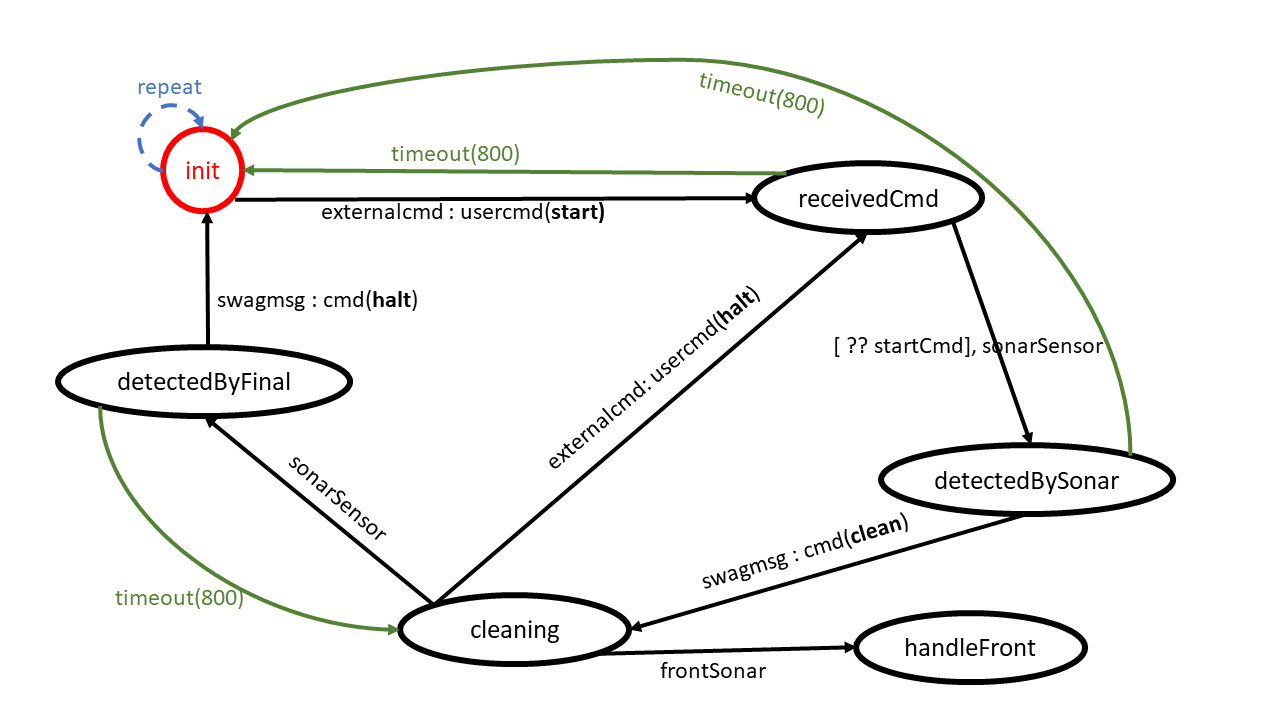
\includegraphics[scale=0.5]{img/stateDiagramStartStopEnd.png}
\caption{ }\labelfig{floorClean1}
\end{figure}

Partendo da questo modello concettuale di base, introduciamo alcuni stati aggiuntivi che derivano dai vincoli imposti dai vincoli specifici del problema.

In particolare consideriamo innanzitutto come il raggiungimento della parete frontale (frontale rispetto alla posizione iniziale del robot, ovvero quella opposta a \code{sonar1}) sia segnalato dalla presenza del secondo sonar, il che consente di rilevare facilmente quando il robot si trova al termine dello stato \codescript{forward}. Da notare come non avvenga niente di analogo per la parete di fondo, dove non abbiamo altro modo se non il sonar frontale del robot a rilevare la presenza di un generico ostacolo.

Quando l'agent, durante lo stato \codescript{forward}, 

\subsection{Obstacle avoidance}
Il \texttt{SoftwareAgent} deve mettersi in ascolto degli eventi \codescript{frontSonar} generati dal sonar frontale del robot quando questi rileva un ostacolo davanti a sé. Quando ciò avviene, deve capire se si tratta di un ostacolo fisso (una parete) o mobile, e cercare di evitarlo.

Nel primo caso deve provare ad aggirare l'ostacolo prima da una direzione e, in caso di fallimento, dall'altra. Il fallimento è determinato dalla presenza di un nuovo ostacolo che impedisce di proseguire oltre in quella direzione -- se fallisce in entrambe le direzioni, la pulizia termina (\code{R-Obstacle}). Se invece trova un passaggio, dopo averlo superato deve tornare alla stessa altezza a cui si trovava prima dell'ostacolo.

Nel secondo caso si assume che, essendo l'ostacolo mobile, questi si sposti dopo un certo tempo. Il robot può quindi limitarsi ad attendere momentaneamente prima di ritentare il passaggio.
%===========================================================================

%===========================================================================
\section{Implementation}
\labelsec{Implementation}
%===========================================================================

%===========================================================================
\section{Testing}
\labelsec{Testing}
%===========================================================================

%===========================================================================
\section{Maintenance}
\labelsec{Maintenance}
%===========================================================================

%===========================================================================
\section{Deployment}
\labelsec{Deployment}
%===========================================================================
 
%===========================================================================
\section{Author}
\labelsec{Author}
%===========================================================================

\vskip.5cm
%%% \begin{figure}
\begin{tabular}{ | c |  }
\hline
  % after \\: \hline or \cline{col1-col2} \cline{col3-col4} ...
  Photo of the author 
  \\
\hline
   %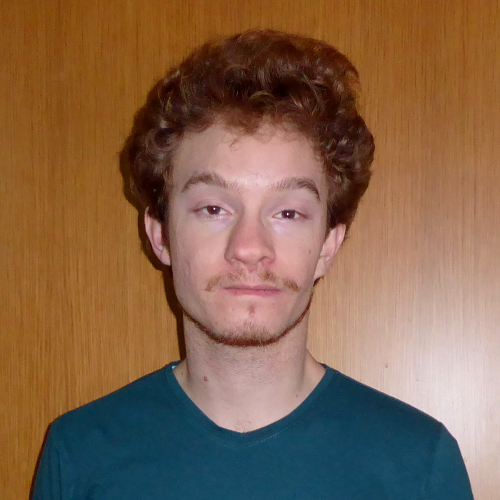
\includegraphics[scale = 0.7]{img/foto_autore.jpg}
   %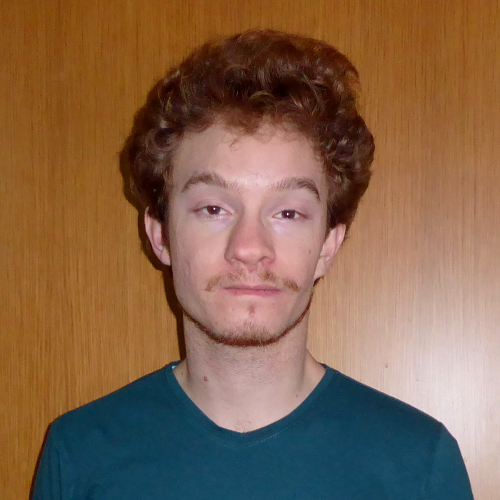
\includegraphics{img/foto_autore.jpg}
  \\
\hline
\end{tabular}
 
\end{document}
